\documentclass[10pt,letter]{article}
\usepackage{amsmath}
\usepackage{amssymb}	% packages that allow mathematical formatting
\usepackage{graphicx}
\graphicspath{{02_Graphs/}}
\usepackage{setspace}	% package that allows you to change spacing
\usepackage{fullpage}	% package that specifies normal margins
\usepackage{microtype}
\usepackage{amsthm}
\newcommand{\argmin}{\operatornamewithlimits{argmin}}
\renewcommand\qedsymbol{$\blacksquare$}
\usepackage{listings,lstautogobble}
\lstset{language=R,
	autogobble=true,
	breaklines=true
}
\usepackage{pgfplotstable} %include csv tables
\usepackage{float} %allows specific table positionings
\usepackage{color}

\definecolor{codegreen}{rgb}{0,0.6,0}
\definecolor{codegray}{rgb}{0.5,0.5,0.5}
\definecolor{backcolour}{rgb}{0.95,0.95,0.95}

\lstdefinestyle{mystyle}{
	backgroundcolor=\color{backcolour},   
	commentstyle=\color{codegreen},
	keywordstyle=\color{blue},
	numberstyle=\tiny\color{codegray},
	stringstyle=\color{cyan},
	basicstyle=\footnotesize,
	breakatwhitespace=false,         
	breaklines=true,                 
	captionpos=b,                    
	keepspaces=true,                 
	numbers=left,                    
	numbersep=5pt,                  
	showspaces=false,                
	showstringspaces=false,
	showtabs=false,                  
	tabsize=2
}

\lstset{style=mystyle}

\usepackage[left=2.5cm, right=2.5cm, top=2cm, bottom = 3cm]{geometry}
	

\begin{document}
\title{FNCE 924 --- Problem Set 2}
\author{Felix Nockher and Patrick Shultz}
\date{\today}
\maketitle 

\section*{Problem a)}

\subsection*{a1) Average growth rate $\gamma$}
We use the following series:

\begin{itemize}
	\item[Y ---] GDPC1: Real GDP Seasonally Adjusted Annual Rate
	\item[I ---] GPDIC1: Real Gross Private Domestic Investment Seasonally Adjusted Annual Rate
	\item[C ---] PCECC96: Real Personal Consumption Expenditures Seasonally Adjusted Annual Rate
\end{itemize}
The average from 1955-Q1 over these three series produces an annual $\gamma_a = 1.0331$ and a quarterly $\gamma_q = \sqrt{\gamma_a} = 1.0082$.

\subsection*{a2) Average capital depreciation rate $\delta$}

We use the following equation:

\begin{align*}
\frac{i}{k} = \frac{(1-\alpha) (\gamma - (1-\delta))}{\frac{1}{\beta}- (1-\delta)}
\end{align*}
which is derived from the FOC w.r.t. capital accumulation in steady state from the detrended problem:

\textbf{detrended}

$$\mathcal{L}= \sum_{t=0}^{\infty} (\beta^\star)^t \lbrace E_0 \left[ u(c,H) + \lambda (Ak^{1-\alpha}H^\alpha-c -k'\gamma + (1-\delta)k )  \right]  $$
where $\lambda = \frac{\Lambda}{\gamma_N}$ and $\beta^\star = \beta \gamma_N$.

\textbf{FOCs}

\begin{align*} \label{FOCs}
[c]\qquad& u_c(c,H) = \lambda \\
[H]\qquad& -u_H(c,H) = \lambda \alpha A k^{1-\alpha} \\
[k']\qquad& 1 = \beta^\star E_0\left[ \frac{\lambda'}{\lambda} \left( (1-\alpha) Ak'^{-\alpha} H'^{\alpha} + 1-\delta \right) \right]\\
[\lambda]\qquad& Ak'^{1-\alpha} H^\alpha  = c+k'-k(1-\delta)
\end{align*}

Then from the Euler equation $[k']$  where in steady state $y=y'$ and $k=k'$ we get
$$\frac{y}{k} = \frac{\frac{1}{\beta}- (1-\delta)}{1-\alpha}$$
Note that we are back to $\beta$ since in the FOC we have $beta^\star/\gamma  $.

\subsection*{a3) Time series for quarterly number of hours worked}
We use the series AWHMAN (Average Weekly Hours of Production and Nonsupervisory Employees: Manufacturing) from FRED. We multiply the weekly figure by four to get monthly values and then add the respective 3 months to generate corresponding quarterly values. The time series mean is 488.3 hours a quarter.

	\begin{figure}[H]
		\centering
		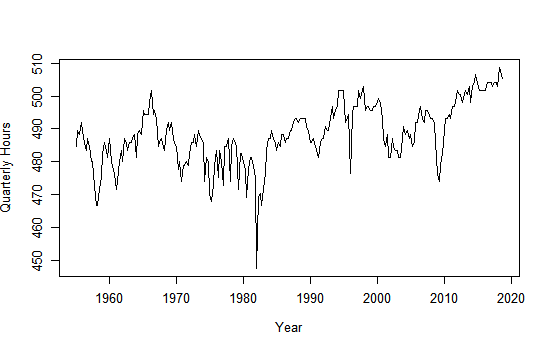
\includegraphics[width=1\linewidth]{A2_Hours.png}
		\caption{Quarterly Number of Hours Worked, $H$}
		\label{fig:QuarterlyHours}
	\end{figure} 

\subsection*{a4) Capital stock}

We use the following equation (perpetual inventory method): $K_{t+1}=I_t+(1-\delta)K_t$:

	\begin{figure}[H]
	\centering
	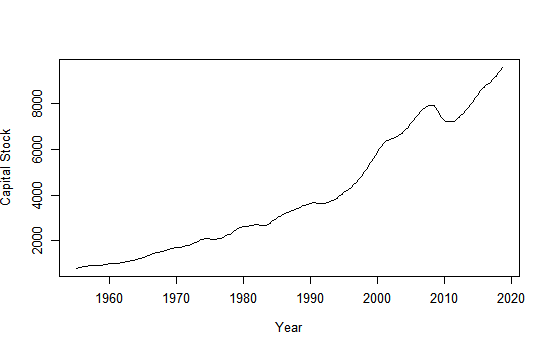
\includegraphics[width=1\linewidth]{A4_CapStock.png}
	\caption{Capital Stock, $K$}
	\label{fig:CapStock}
\end{figure} 

\subsection*{a5) Solow residual (TFP)}
We use CRS with $\alpha = 2/3$ and the following equation: $$log(A)= log(Y)-(1-\alpha)log(K)-\alpha log(H)$$

	\begin{figure}[H]
	\centering
	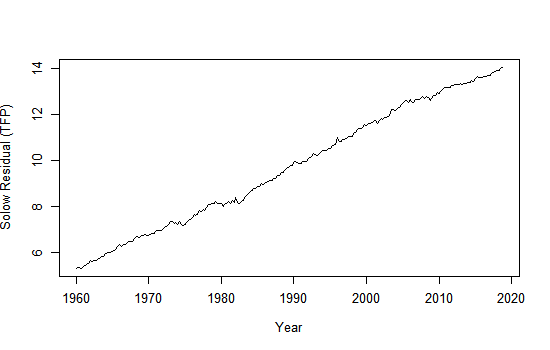
\includegraphics[width=1\linewidth]{A5_SolowRes.png}
	\caption{Solow Residual, $A$}
	\label{fig:SolowRes}
\end{figure} 

\section*{Problem b)}
We detrended the log of the series of Y, I, C, K, and H via the HP filter and a frequency of 1600. Note that we also used the filter for the H series to get the cycle component only even though the series has no actual trend.
\subsection*{b1) Second moments}
For the filtered series we get:
	
% Table created by stargazer v.5.2.2 by Marek Hlavac, Harvard University. E-mail: hlavac at fas.harvard.edu
% Date and time: Sun, Apr 14, 2019 - 7:00:14 PM
\begin{table}[!htbp] \centering 
  \caption{Comparing Second Moments} 
  \label{TableB1} 
\begin{tabular}{@{\extracolsep{5pt}} ccccc} 
\\[-1.8ex]\hline 
\hline \\[-1.8ex] 
 & y & c & i & h \\ 
\hline \\[-1.8ex] 
Sigma(.) & 1.44658277806168 & $1.176$ & $6.541$ & $1.044$ \\ 
Sigma(.)/Sigma(y) &  & $0.813$ & $4.521$ & $0.722$ \\ 
Rho(.,y) &  & $0.871$ & $0.901$ & $0.670$ \\ 
\hline \\[-1.8ex] 
\end{tabular} 
\end{table} 
 %


\subsection*{b2/b3) AR(2)/AR(1) process for the Solow Residual}


% Table created by stargazer v.5.2.2 by Marek Hlavac, Harvard University. E-mail: hlavac at fas.harvard.edu
% Date and time: Sun, Apr 14, 2019 - 7:00:15 PM
\begin{table}[!htbp] \centering 
  \caption{Autoregression} 
  \label{TableB2} 
\begin{tabular}{@{\extracolsep{5pt}} ccccc} 
\\[-1.8ex]\hline 
\hline \\[-1.8ex] 
 & Coeff & tstat & Rho\_a & sigma\_a \\ 
\hline \\[-1.8ex] 
AR(2)-1 & $0.526$ & $8.108$ &  &  \\ 
AR(2)-2 & $0.126$ & $1.953$ &  &  \\ 
AR(1)-1 & $0.601$ & $11.591$ & 0.601481835416286 & 0.00662892932563865 \\ 
\hline \\[-1.8ex] 
\end{tabular} 
\end{table} 
 %
We see that we are very close to rejecting the null of $\varphi_2 = 0$ to the $5\%$ level with a t-stat of 1.95. We reject the null that the $varphi_1$ is zero to the $1\%$ level for both suggested processes.
The standard deviation for the AR(1) innovation, $\sigma_a$ is approx. $0.6\%$.

\section*{Problem c)}
\subsection*{c1) FOCs for KPR preferences}
Note that the general outline of the detrended problem can be found in Equation \eqref{FOCs}. We plug in the respective derivatives w.r.t. $c$ and $H$ of $u(c,H)=log(c)+\psi log(1-H)$:

\begin{align*}
[c]\qquad& \frac{1}{c} = \lambda \\
[H]\qquad& -(-\frac{1}{1-H}\psi) = \lambda \alpha A k^{1-\alpha} \\
[k']\qquad& 1 = \beta^\star E_0\left[ \frac{\lambda'}{\lambda} \left( (1-\alpha) Ak'^{-\alpha} H'^{\alpha} + 1-\delta \right) \right]\\
[\lambda]\qquad& Ak'^{1-\alpha} H^\alpha  = c+k'-k(1-\delta)
\end{align*}

\subsection*{c2) Calibrate for $\psi$} \label{c2}
We use the FOC w.r.t. hours worked, $H$, and replace $\lambda$ via the FOC w.r.t. $c$ and note that $Ak^{1-\alpha} H^{\alpha-1}\alpha = \frac{y}{H}\alpha$:
$$\psi = \frac{1-H}{H}\frac{Y}{H} = \frac{1-H}{H}\frac{y}{c}\alpha$$
Note that we first calculated the daily average of H by dividinng it by $(3months*4weeks*7days*24h)$ such that is a percentage number of hours worked per day. We then calculate both fractions over time and then plug in the average over time to get $psi = 3.24$.

\section*{e) GHH preferences}
The partials of the GHH utility are:

\begin{align*}
u_C& = \frac{1}{C-\psi\frac{H^{1+\nu}}{1+\nu}}\\
u_H& = \frac{-\psi H^\nu}{C-\psi frac{H^{1+\nu}}{1+\nu}}
\end{align*}

As in Subsection \ref{c2} we then use the FOC of the problem w.r.t. hours worked, this time not debased to a percentage figure, and replace $\lambda$ via the result of the FOC w.r.t. consumption:
$$\psi = \frac{1}{H^\nu}\frac{Y}{H} \alpha$$

We detrend Y over time by dividing it by population (both in the same units, i.e. Y upscaled from billions), deploying $\nu = 0.5$, and taking the time series average of the ratio to get $\psi = 3.65$.


% Table created by stargazer v.5.2.2 by Marek Hlavac, Harvard University. E-mail: hlavac at fas.harvard.edu
% Date and time: Sun, Apr 14, 2019 - 7:00:14 PM
\begin{table}[!htbp] \centering 
  \caption{Comparing Second Moments} 
  \label{TableB1} 
\begin{tabular}{@{\extracolsep{5pt}} ccccc} 
\\[-1.8ex]\hline 
\hline \\[-1.8ex] 
 & y & c & i & h \\ 
\hline \\[-1.8ex] 
Sigma(.) & 1.44658277806168 & $1.176$ & $6.541$ & $1.044$ \\ 
Sigma(.)/Sigma(y) &  & $0.813$ & $4.521$ & $0.722$ \\ 
Rho(.,y) &  & $0.871$ & $0.901$ & $0.670$ \\ 
\hline \\[-1.8ex] 
\end{tabular} 
\end{table} 
 %
\section*{d) Use Dynare to solve the model}
We define the equations in our model as 
\begin{enumerate}
	\item $\frac{1}{c_t} = \lambda_t$
	\item $\gamma = \beta^{\star}E_t\left[\dfrac{c_{t}}{c_{t+1}}\bigg((1-\alpha)A_{t+1} k_{t+1}^{-\alpha}H_{t+1}^{\alpha} + (1-\delta)\bigg)\right]$
	\item $\dfrac{\psi}{1-H_{t}} = \dfrac{1}{c_{t}}\left(\alpha A_{t}k_{t}^{1-\alpha}H_{t}^{\alpha-1}\right)$
	\item $A_{t}k_{t}^{1-\alpha}H_{t}^{\alpha} + (1-\delta)k_{t}-k_{t+1}\gamma = c_{t}$
	\item $\log A_{t+1} = \rho A_{t} + \sigma_{A}\epsilon$
    \item $y_{t} = A_{t}k_{t}^{1-\alpha}H_{t}^{\alpha}$
    \item $y_{t} = c_{t} + i_{t}$
    \item $w_{t} = \alpha A_{t}k_{t}^{1-\alpha}H_{t}^{\alpha-1}$
    \item $r_t = (1-\alpha)A_{t}k_{t}^{\alpha}$
\end{enumerate}  
We then solve for the steady states of nine unknowns: $r, i, y, c, w, \bar{a}, \psi, \lambda, k$. We can also use the equations above to solve for the deterministic steady state values that will be used as initial values in dynare. Figure \ref{fig:KPR_irfs} displays the impulse response functions for output, consumption, investment, and hours to a positive TFP shock. \\

\begin{figure}[H]
	\centering
	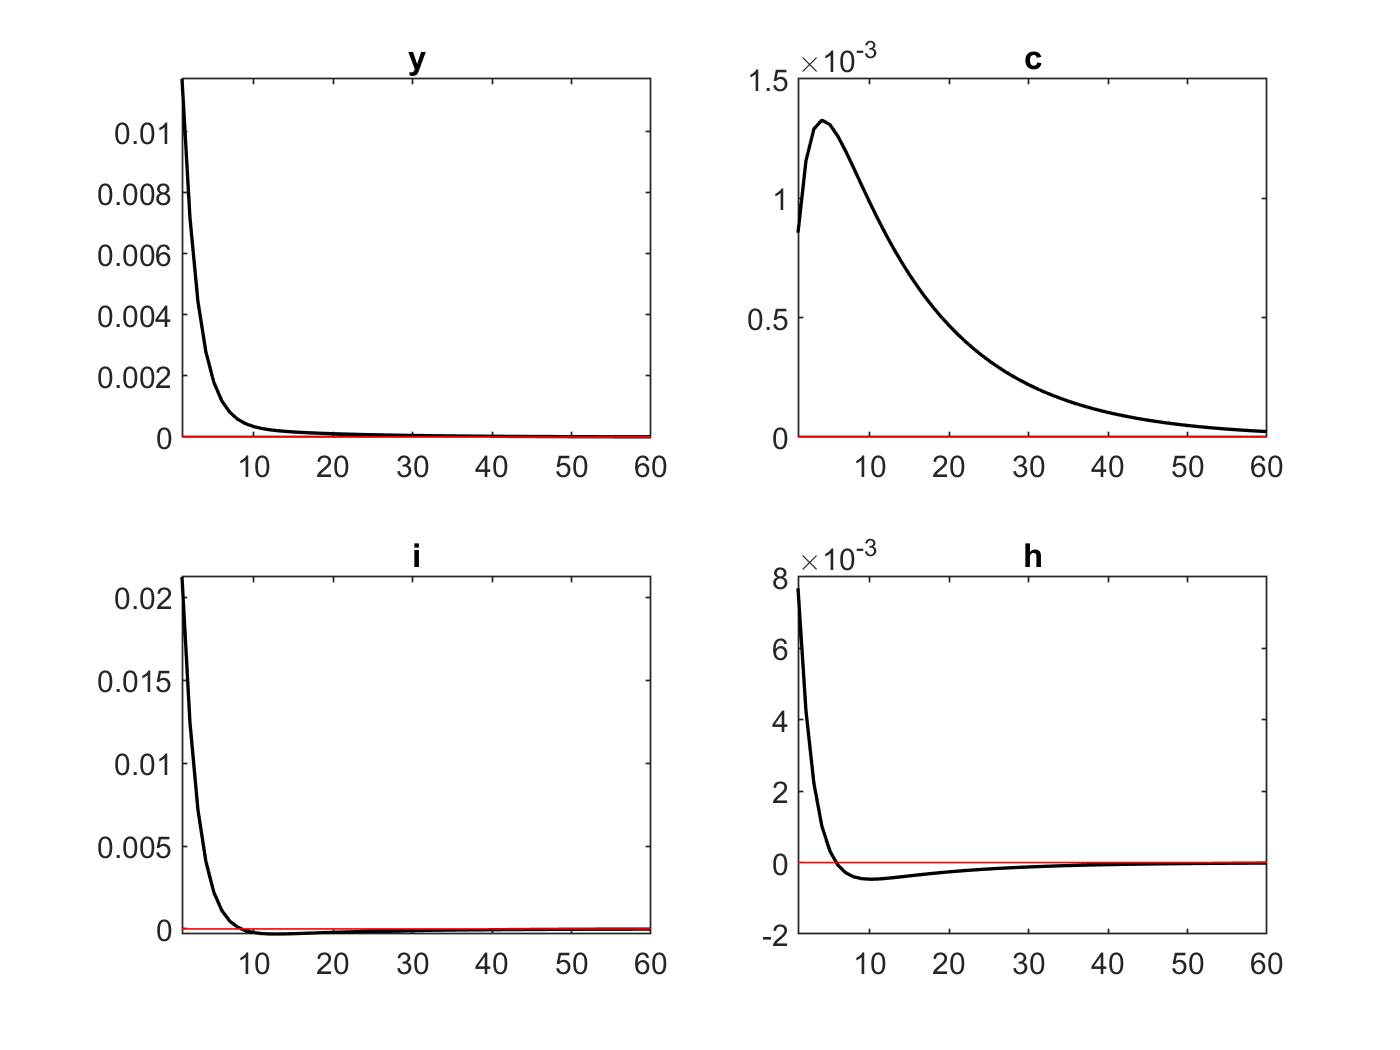
\includegraphics[width=1\linewidth]{irfs_yich_kpr.png}
	\caption{Impulse responses of output, consumption, investment, and hours to a positive TFP shock using KPR preferences}
	\label{fig:KPR_irfs}
\end{figure} 


\begin{table}[H]
	\centering
	\begin{tabular}{l|lll}
		Variable & $\sigma(\cdot)$ & $\sigma(\cdot)/\sigma(y)$ \\\hline
				$y$ & 0.0126 & 1    &  \\
				$i$ & 0.0229 & 1.82 &  \\
				$c$ & 0.0018 & 0.14 &  \\
				$h$ & 0.0084 & 0.66 &  \\
				$w$ & 0.0044 & 0.35 &  
	\end{tabular}
\caption{Standard deviations of relevant variables}
\end{table}
Comparing to Table \ref{TableB1}, we see that the model matches the variance of output and  hours well. However, the model fails to capture the volatiltiy of investment and consumption. When looking at the ratio of the standard deviations relative to output, we see that the model captures the relative variances of hours worked and investment, but misses the fact that consumption is less volatile than output.

\begin{table}[H]
	\centering
	\begin{tabular}{l|lllll}
		Order  & 1      & 2      & 3       & 4       & 5       \\\hline
		a      & 0.4653 & 0.1538 & -0.0220 & -0.1153 & -0.1587 \\
		y      & 0.4699 & 0.1596 & -0.0167 & -0.1113 & -0.1563 \\
		i      & 0.4612 & 0.1486 & -0.0268 & -0.1189 & -0.1610 \\
		k      & 0.8978 & 0.7029 & 0.4797  & 0.2639  & 0.0738  \\
		c      & 0.8755 & 0.6747 & 0.4539  & 0.2444  & 0.0619  \\
		h      & 0.4547 & 0.1404 & -0.0343 & -0.1246 & -0.1644 \\
		r      & 0.4536 & 0.1389 & -0.0356 & -0.1256 & -0.1650 \\
		w      & 0.5390 & 0.2473 & 0.0634  & -0.0508 & -0.1191 \\
		lambda & 0.8755 & 0.6747 & 0.4539  & 0.2444  & 0.0619 
	\end{tabular}
\caption{Autocorrelations}
\end{table}

\begin{table}[H]
	\centering
	\begin{tabular}{l|lllllllll}
		Variables & a       & y       & i       & k       & c       & h       & r       & w       & $\lambda$  \\\hline
		a         & 1.0000  & 0.9996  & 0.9995  & 0.3797  & 0.4625  & 0.9946  & 0.9820  & 0.9609  & -0.4625 \\
		y         & 0.9996  & 1.0000  & 0.9983  & 0.4059  & 0.4876  & 0.9912  & 0.9762  & 0.9684  & -0.4876 \\
		i         & 0.9995  & 0.9983  & 1.0000  & 0.3514  & 0.4353  & 0.9973  & 0.9873  & 0.9520  & -0.4353 \\
		k         & 0.3797  & 0.4059  & 0.3514  & 1.0000  & 0.9958  & 0.2815  & 0.1981  & 0.6211  & -0.9958 \\
		c         & 0.4625  & 0.4876  & 0.4353  & 0.9958  & 1.0000  & 0.3678  & 0.2866  & 0.6900  & -1.0000 \\
		h         & 0.9946  & 0.9912  & 0.9973  & 0.2815  & 0.3678  & 1.0000  & 0.9963  & 0.9269  & -0.3678 \\
		r         & 0.9820  & 0.9762  & 0.9873  & 0.1981  & 0.2866  & 0.9963  & 1.0000  & 0.8912  & -0.2866 \\
		w         & 0.9609  & 0.9684  & 0.9520  & 0.6211  & 0.6900  & 0.9269  & 0.8912  & 1.0000  & -0.6900 \\
		$\lambda$    & -0.4625 & -0.4876 & -0.4353 & -0.9958 & -1.0000 & -0.3678 & -0.2866 & -0.6900 & 1.0000 
	\end{tabular}
\caption{Correlations}
\end{table}
\section*{e)}
We now assume that preferences take the form
\begin{equation*}
	u(C, L) = \log \left(C - \psi \dfrac{H^{1+\nu}}{1+\nu}\right)
\end{equation*}
Our model becomes 
\begin{enumerate}
	\item $\frac{1}{c_t-\psi \dfrac{H_{t}^{1+\nu}}{1+\nu}} = \lambda_t$
	\item $\gamma = \beta^{\star}E_t\left[\dfrac{\lambda_{t+1}}{\lambda_{t}}\bigg((1-\alpha)A_{t+1} k_{t+1}^{-\alpha}H_{t+1}^{\alpha} + (1-\delta)\bigg)\right]$
	\item $\psi H_{t}^{\nu} = \alpha A_{t}k_{t}^{1-\alpha}H_{t}^{\alpha-1}$
	\item $A_{t}k_{t}^{1-\alpha}H_{t}^{\alpha} + (1-\delta)k_{t}-k_{t+1}\gamma = c_{t}$
	\item $\log A_{t+1} = \rho A_{t} + \sigma_{A}\epsilon$
	\item $y_{t} = A_{t}k_{t}^{1-\alpha}H_{t}^{\alpha}$
	\item $y_{t} = c_{t} + i_{t}$
	\item $w_{t} = \alpha A_{t}k_{t}^{1-\alpha}H_{t}^{\alpha-1}$
	\item $r_t = (1-\alpha)A_{t}k_{t}^{\alpha}$
\end{enumerate}
\begin{figure}[H]
	\centering
	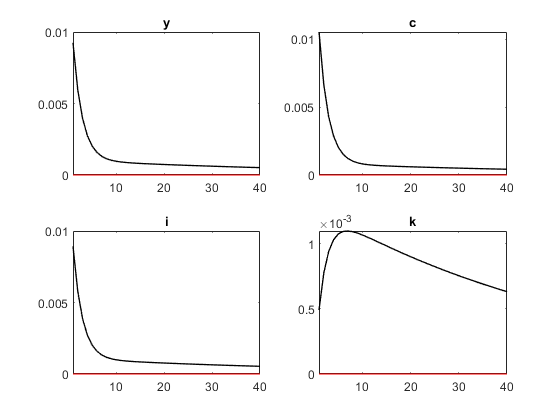
\includegraphics[width=1\linewidth]{irfs_yich_ghh.png}
	\caption{Impulse responses of output, consumption, investment, and hours to a positive TFP shock using GHH preferences}
	\label{fig:GHH_irfs}
\end{figure} 

\begin{table}[H]
	\centering
	\begin{tabular}{l|lll}
		Variable & $\sigma(\cdot)$ & $\sigma(\cdot)/\sigma(y)$ \\\hline
	$y$ & 0.00982 & 1     \\
	$i$ & 0.00948 & 0.965 \\
	$c$ & 0.011   & 1.1   \\
	$h$ & 0.0085  & 0.86  \\
	$w$ & 0.0042  & 0.43  
\end{tabular}
\caption{Standard deviations of relevant variables}
\end{table}
\begin{table}[H]
	\centering
	\begin{tabular}{l|lllll}
	Order  & 1      & 2      & 3       & 4       & 5       \\\hline
	a      & 0.4653 & 0.1538 & -0.0220 & -0.1153 & -0.1587 \\
	y      & 0.4732 & 0.1640 & -0.0125 & -0.1079 & -0.1539 \\
	i      & 0.4743 & 0.1653 & -0.0113 & -0.1070 & -0.1533 \\
	k      & 0.9041 & 0.7192 & 0.5050  & 0.2951  & 0.1075  \\
	c      & 0.4701 & 0.1600 & -0.0162 & -0.1108 & -0.1558 \\
	h      & 0.4689 & 0.1584 & -0.0178 & -0.1120 & -0.1566 \\
	r      & 0.4646 & 0.1529 & -0.0229 & -0.1160 & -0.1592 \\
	w      & 0.4689 & 0.1584 & -0.0178 & -0.1120 & -0.1566 \\
	$\lambda$ & 0.9260 & 0.7474 & 0.5313  & 0.3156  & 0.1208 
	\end{tabular}
	\caption{Autocorrelations}
\end{table}

\begin{table}[]
	\begin{tabular}{l|lllllllll}
		Variables & a       & y       & i       & k       & c       & h       & r       & w      & $\lambda$  \\\hline
		a         & 1.0000  & 0.9952  & 0.9944  & 0.2572  & 0.9975  & 0.9984  & 0.9993  & 0.9984 & -0.0165 \\
		y         & 0.9952  & 1.0000  & 1.0000  & 0.3503  & 0.9996  & 0.9992  & 0.9909  & 0.9992 & -0.1141 \\
		i         & 0.9944  & 1.0000  & 1.0000  & 0.3578  & 0.9994  & 0.9988  & 0.9898  & 0.9988 & -0.1220 \\
		k         & 0.2572  & 0.3503  & 0.3578  & 1.0000  & 0.3245  & 0.3116  & 0.2211  & 0.3116 & -0.9705 \\
		c         & 0.9975  & 0.9996  & 0.9994  & 0.3245  & 1.0000  & 0.9999  & 0.9942  & 0.9999 & -0.0867 \\
		h         & 0.9984  & 0.9992  & 0.9988  & 0.3116  & 0.9999  & 1.0000  & 0.9956  & 1.0000 & -0.0732 \\
		r         & 0.9993  & 0.9909  & 0.9898  & 0.2211  & 0.9942  & 0.9956  & 1.0000  & 0.9956 & 0.0207  \\
		w         & 0.9984  & 0.9992  & 0.9988  & 0.3116  & 0.9999  & 1.0000  & 0.9956  & 1.0000 & -0.0732 \\
		$\lambda$    & -0.0165 & -0.1141 & -0.1220 & -0.9705 & -0.0867 & -0.0732 & -0.0732 & 0.3156 & 0.1208 
	\end{tabular}
\caption{Correlations}
\end{table}
\section*{f) Government expenditure} \label{c2}

\subsection*{f1) Time series average G/Y}
We use the quarterly FRED series W068RCQ027SBEA (Government total expenditures - Seasonally adjusted annual rate). We get a time series average of $\frac{G}{Y} = 20.0\%$ for the data since inception, i.e. 1960-Q1.

\subsection*{f2) AR(1) of the HP filtered series}


% Table created by stargazer v.5.2.2 by Marek Hlavac, Harvard University. E-mail: hlavac at fas.harvard.edu
% Date and time: Sun, Apr 14, 2019 - 8:38:21 PM
\begin{table}[!htbp] \centering 
  \caption{Government Autoregression} 
  \label{Tablef2} 
\begin{tabular}{@{\extracolsep{5pt}} cccc} 
\\[-1.8ex]\hline 
\hline \\[-1.8ex] 
 & rho\_g & t\_stat\_g & sigma\_g \\ 
\hline \\[-1.8ex] 
 & $0.785$ & $19.407$ & $0.010$ \\ 
\hline \\[-1.8ex] 
\end{tabular} 
\end{table} 
 %




\section*{Appendix - Code}
\subsection*{Data preparation}
%\lstinputlisting{../Code/190414_Data_preparation_v08.R}

\end{document}